\section{Different approaches of vision tasks}
\label{sec:differentApproaches}

Many different kinds of vision tasks input image data.
These use cases outline broad guidelines for designing neural network architectures and the workflow of such a model by which the desired output is produced.
\autoref{fig:differentApproaches} shows the outputs of the most commonly used strategies in the literature that might be relevant for rail track prediction or a part of it.
The input image for all models is visualized in \autoref{fig:differentApproaches_classification} without the added text in the top right corner.

\vspace{1cm} % Größerer Abstand zwischen den Reihen

\begin{figure}[H]
    \centering
    
    % Erste Reihe
    \begin{subfigure}{0.328\textwidth}
        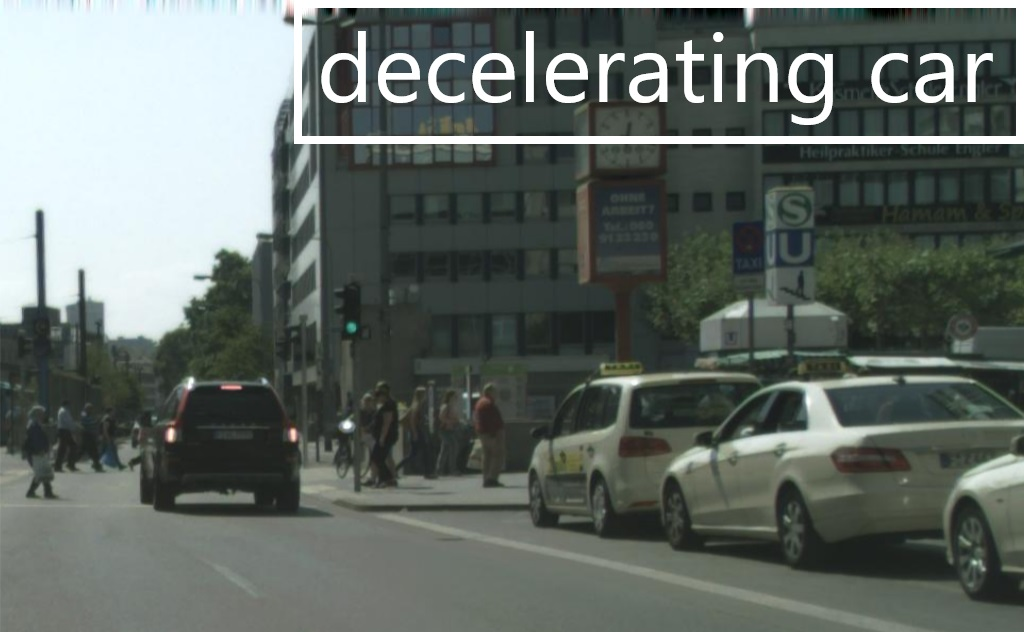
\includegraphics[width=\linewidth]{PICs/differentApproaches/classification_v2.jpg}
        \caption{classification}
        \label{fig:differentApproaches_classification}
    \end{subfigure}
    \hfill
    \begin{subfigure}{0.328\textwidth}
        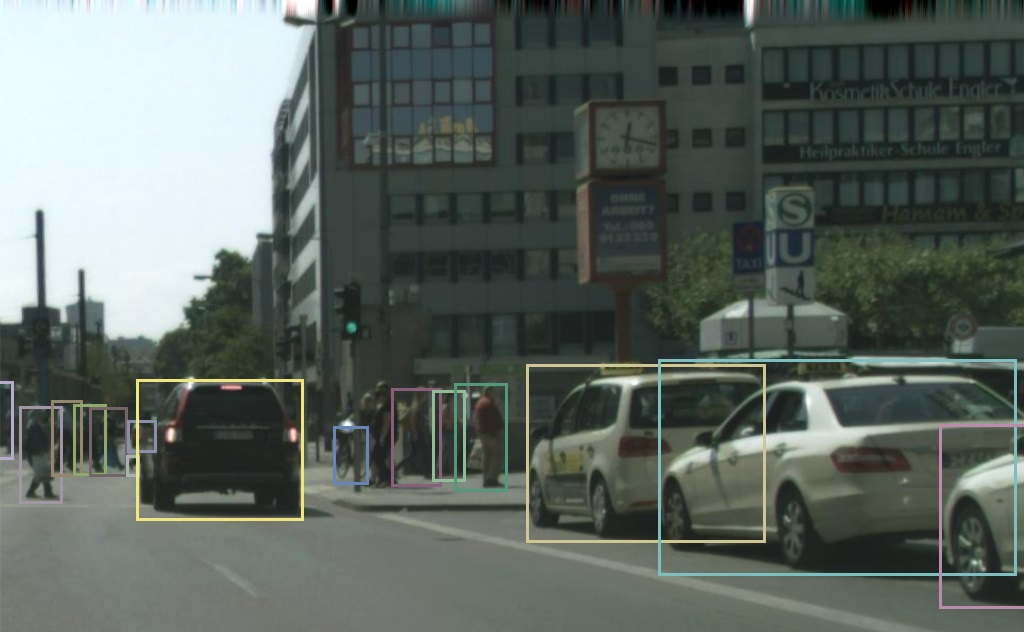
\includegraphics[width=\linewidth]{PICs/differentApproaches/object_detection.jpg}
        \caption{object detection}
        \label{fig:differentApproaches_object_detection}
    \end{subfigure}
    \hfill
    \begin{subfigure}{0.328\textwidth}
        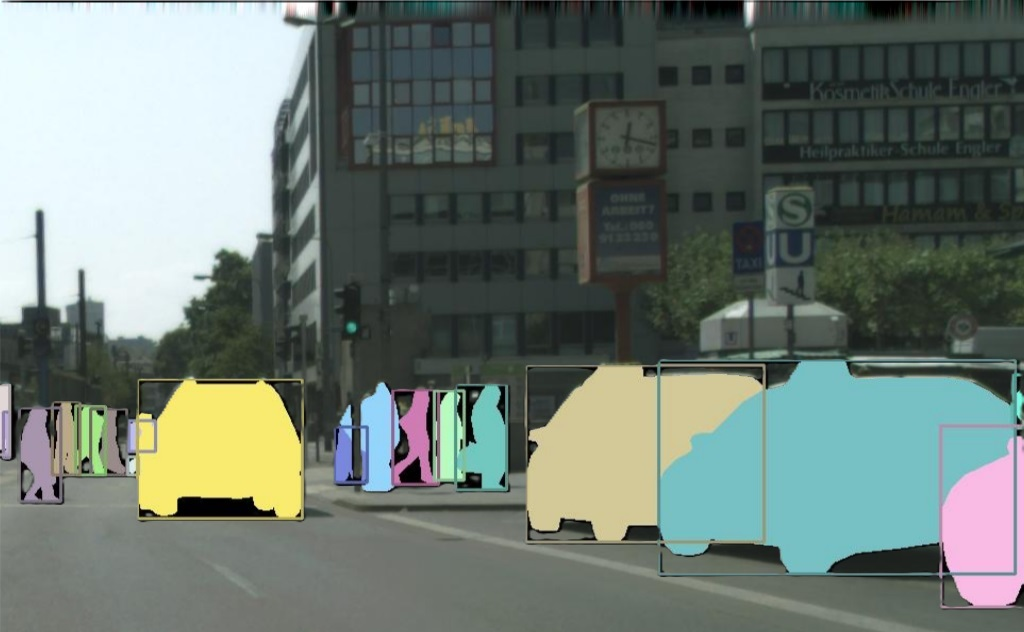
\includegraphics[width=\linewidth]{PICs/differentApproaches/instance_segmentation_v2.jpg}
        \caption{instance segmentation}
        \label{fig:differentApproaches_instance_segmentation}
    \end{subfigure}

    \vspace{0.1cm} % Größerer Abstand zwischen den Reihen

    % Zweite Reihe
    \begin{subfigure}{0.328\textwidth}
        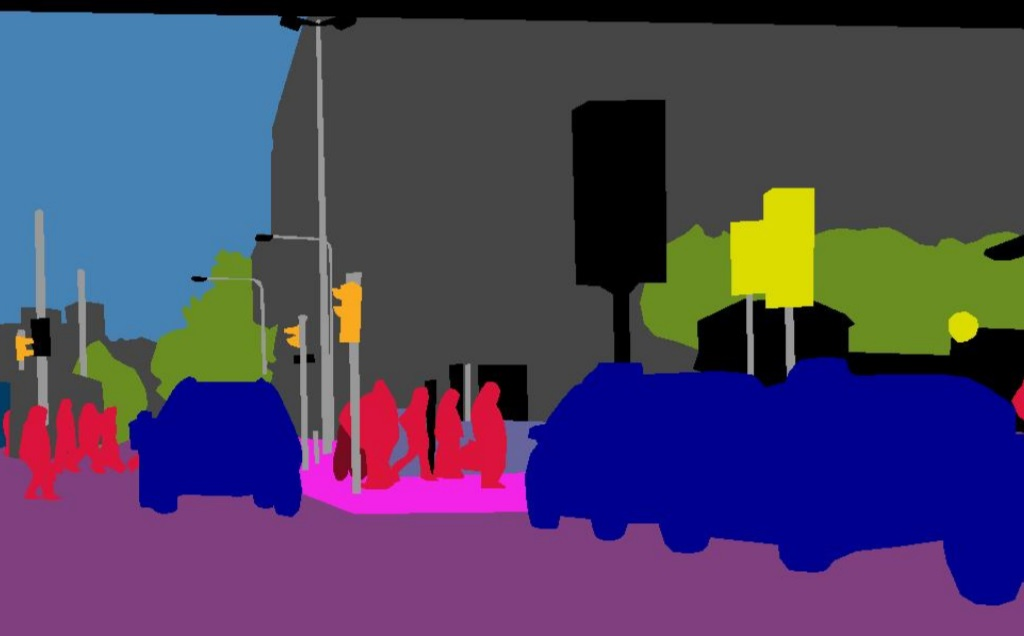
\includegraphics[width=\linewidth]{PICs/differentApproaches/semantic_segmentation.jpg}
        \caption{semantic segmentation}
        \label{fig:differentApproaches_semantic_segmentation}
    \end{subfigure}
    \hfill
    \begin{subfigure}{0.328\textwidth}
        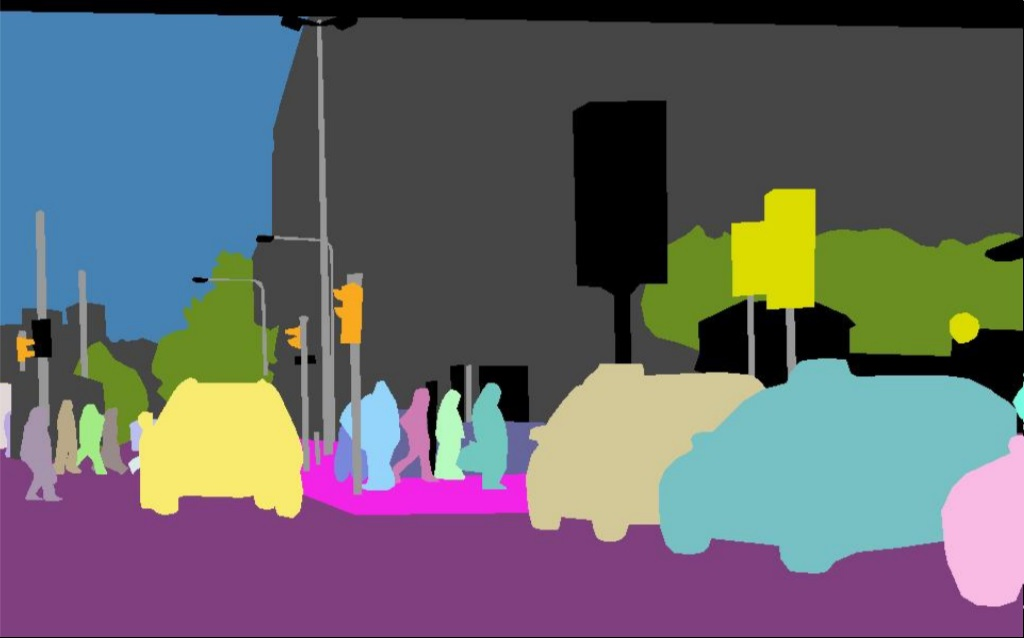
\includegraphics[width=\linewidth]{PICs/differentApproaches/panoptic_segmentation.jpg}
        \caption{panoptic segmentation}
        \label{fig:differentApproaches_panoptic_segmentation}
    \end{subfigure}
    \hfill
    \begin{subfigure}{0.328\textwidth}
        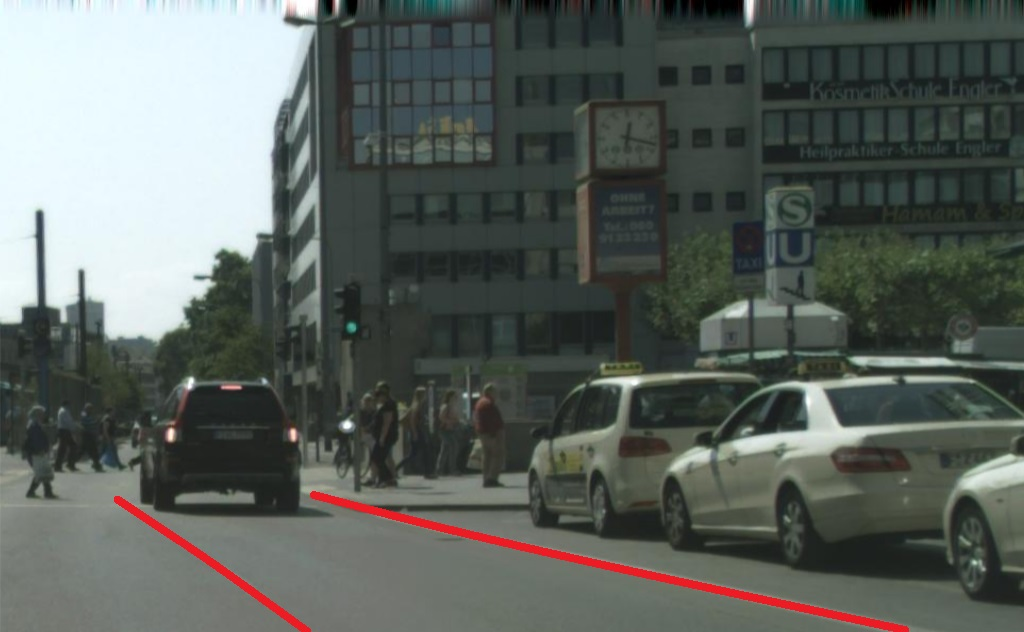
\includegraphics[width=\linewidth]{PICs/differentApproaches/line_detection.jpg}
        \caption{line detection}
        \label{fig:differentApproaches_line_detection}
    \end{subfigure}

    \caption{The most common applications in vision tasks that are supported by neural networks. Shown are \ac{GT} examples for each usage domain. The input image is visualized in (a) without the added text in the top right corner \cite{panopticsegmentation2019}.}
    \label{fig:differentApproaches}
\end{figure}

\noindent\textbf{Classification} describes the scene in the input image with only one label.
\autoref{fig:differentApproaches_classification} shows a possible example with the label added in the top right corner of the input image.
No further information is available from the output of a classification method \cite{cifar100}.

\vspace{1cm} % Größerer Abstand zwischen den Reihen

\noindent\textbf{Object detection} combines classification with localization.
This technique outputs so-called bounding boxes that also include positional information of objects.
Additionally, class labels are assigned to each bounding box, which show what has been recognized \cite{panopticsegmentation2019}.

\vspace{1cm} % Größerer Abstand zwischen den Reihen

\noindent\textbf{Instance segmentation} expands on object detection by not just outputting bounding boxes.
It generates binary masks within each bounding box, enabling more accurate identification of the pixels that belong to the object and those that do not.
Regions within the bounding box that are not part of the object are disregarded \cite{panopticsegmentation2019}.

\vspace{1cm} % Größerer Abstand zwischen den Reihen

\noindent\textbf{Semantic segmentation} is a method that outputs a class label for each pixel of the input image.
Consequently, the output consists of a mask with the same width and height as the input image.
An example is shown in \autoref{fig:differentApproaches_semantic_segmentation} with people and cars being two of the output labels.
In this work, semantic segmentation can be used for filtering out the rail track, for example \cite{panopticsegmentation2019}.

\vspace{1cm} % Größerer Abstand zwischen den Reihen

\noindent\textbf{Panoptic segmentation} combines semantic segmentation and instance segmentation.
It makes the difference between so-called "things" and "stuff" \cite{panopticsegmentation2019}.
Examples of "things" in \autoref{fig:differentApproaches_panoptic_segmentation} are countable objects like cars and people.
Examples of "stuff" are the road, buildings, or the sky.
As with semantic segmentation, this method outputs a pixel-wise classification.
This mask also has the same dimensions as the input image.
However, while semantic segmentation assigns the same class to different instances of the same objects, panoptic segmentation can differentiate between different "things".
\autoref{fig:differentApproaches_panoptic_segmentation} shows that each car or person has its unique class label.

\vspace{1cm} % Größerer Abstand zwischen den Reihen

\noindent\textbf{Line detection} algorithms are usually tailored to filter out lines like road markings or rails.
\autoref{fig:differentApproaches_line_detection} shows a possible output in the road domain of such an algorithm.
Even though in the field of line detection a lot of work has been done in the road domain, this work mainly focuses on applications in the rail domain.
Furthermore, many state-of-the-art papers include outputs in the form of binary masks with the same dimensions as the input image.
While these models solve the line detection problem, they use pixel-wise classification and technically fall into the category of semantic segmentation.
In this work, these papers are therefore reviewed in the corresponding section.
Solely techniques not based on semantic segmentation are included in the line detection section.

\vspace{2cm} % Größerer Abstand zwischen den Reihen

\noindent Following a brief description of all the various approaches, it becomes clear that only object detection, semantic segmentation, and line detection are viable options for rail track prediction.
Object detection can be used to filter out switches in the image and their states.
The information on whether a switch state is left or right can be useful for predicting the leading rail in an application.
Semantic segmentation can be used to identify the track itself on the pixel level.
This solution provides a more intuitive solution for train operators where not only a state is outputted, but the track is visualized in the image.
Ideally, object detection and track segmentation are combined to display only the train's track.
The third approach, which must not be overlooked, is line detection algorithms.
While the output and techniques slightly differ from semantic segmentation, they also provide important pixel-wise information about the track.
As the other approaches are not suitable or relevant for this use case, they are excluded. The following sections focus on the three techniques mentioned and describe them in more detail.